\documentclass[a4paper]{article}
\usepackage[spanish]{babel}

\usepackage[utf8]{inputenc}
\usepackage{amsmath}
\usepackage{esvect}
\usepackage{graphicx,caption}%
\usepackage[colorinlistoftodos]{todonotes}
\usepackage[]{comment}
\usepackage{booktabs}
\usepackage{caption}
\usepackage{subcaption}
% \usepackage{booktabs}
\usepackage{graphicx}
\usepackage{graphicx,wrapfig,lipsum}
\usepackage{geometry}
 \geometry{
 a4paper,
 total={170mm,257mm},
 left=20mm,
 top=20mm,
 }
\title{Ejercicio 7 Practica 2 - Regresion Lineal(Parte 2)}
\author{Rafael Barrera Oro, Grover Aruquipa}
\date{31-05-2021}
\begin{document}


\maketitle

\newpage


\newpage



\section{Resolución}
Link de codigo fuente: $https://github.com/GroverAruquipa/Works\_Aprendizaje\_estadistico\_UBA$

\subsection{Punto 1}
\footnote{El codigo fuente se puede encontrar en \url{https://github.com/GroverAruquipa/Works_Aprendizaje_estadistico_UBA}.}

Estimamos la matriz de correlación para todas las variables:

\begin{center}
    \begin{tabular}{|c|c|c|c|c|c|c|c|}
        \hline
                        & \textbf{X1}   & \textbf{X2}   & \textbf{X3}   & \textbf{X4}   & \textbf{X5} &\textbf{Y}\\
        \hline            
        \textbf{X1}     & 1         &  -0.84       &    -0.24      &    0.14      & -0.35     & -0.64  \\
        \hline
        \textbf{X2}     & -0.84      & 1     & 0.33    &    -.034   & 0.34    & 0.76   \\
        \hline
        \textbf{X3}     & -0.24     &  0.33    & 1  & -0.98     & 0.21  & 0.85  \\
        \hline
        \textbf{X4}     &   0.14   & -0.34   &  -0.98 & 1    & -0.22     & -0.83   \\
        \hline
        \textbf{X5}     &   -0.35   &   0.34    &    0.21  &    -0.22 & 1     & 0.33   \\
        \hline
        \textbf{Y}      &   -0.64   &   0.76  & 0.85&   -0.83   &   0.33   & 1     \\
        \hline
    \end{tabular}
\end{center}
De esta forma en las figuras \ref{fig:corr1} y \ref{fig:corr2} son mostrados los graficos de correlacion entre variables.
\begin{figure}[h]
     \centering
     \begin{subfigure}[b]{0.4\textwidth}
         \centering
         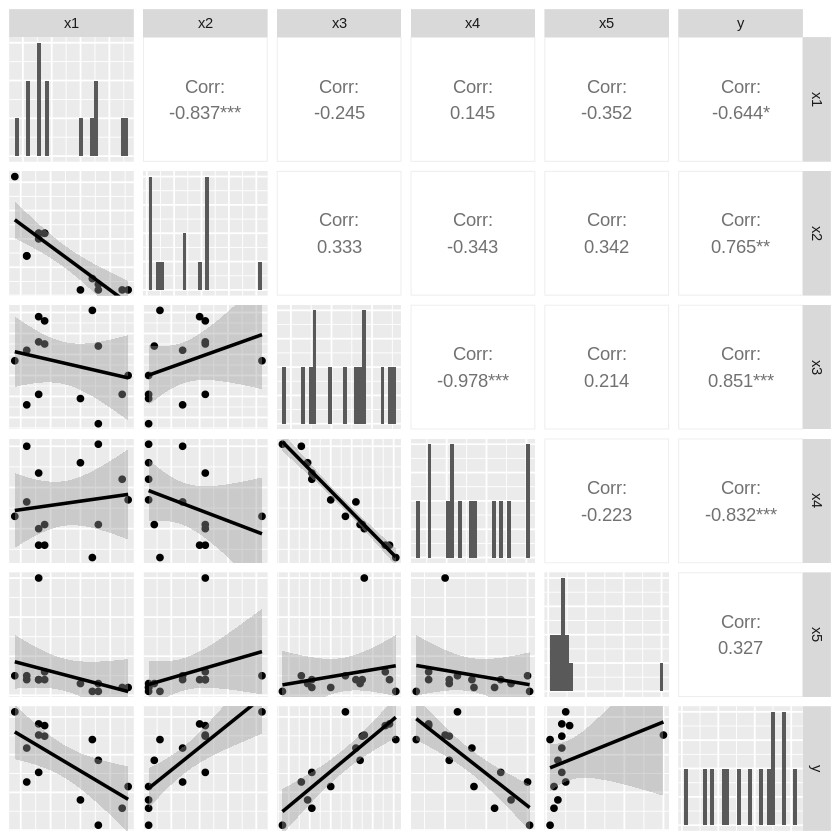
\includegraphics[width=\textwidth]{pc1.jpg}
         \caption{Matriz de correlacion numerica.}
         \label{fig:corr1}
     \end{subfigure}
     \hfill
     \begin{subfigure}[b]{0.4\textwidth}
         \centering
         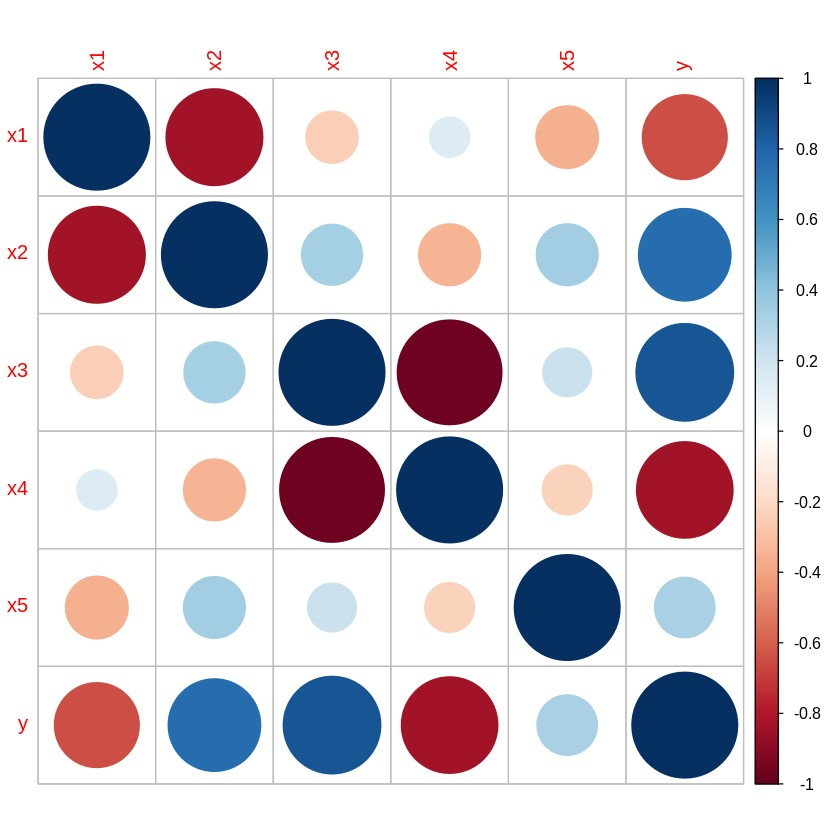
\includegraphics[width=\textwidth]{pr2.jpg}
         \caption{Matriz de correlacion grafica.}
         \label{fig:corr2}
     \end{subfigure}
     \hfill
        \caption{Graficos de correlacion.}
        \label{fig:three graphs}
\end{figure}
De la matriz de correlacion se puede indicar que las variables con mayor correlacion respecto a \textbf{Y}  es \textbf{$x_4$} con 0.832 y \textbf{$x_3$} con 0.851. De igual froma las variables \textbf{$x_3$} y \textbf{$x_4$} tiene una alta correlacion de 0.978 lo que indica que puede ser simplificado en una sola en un futuro.


\subsection{Punto 2}
Para el ajuste lineal con la variable \textbf{Y} y un intercept fueron econtrados los siguientes resultados:\\
\begin{equation}
    Y=73.61-0.449*x_1+1.299*x_2+0.563*x_3-0.17*x_4-0.386*x_5
    \label{modelo1}
\end{equation}
Un error cuadratico de $0.9871$, un error cuadratico ajustado de $0.9760$ y un p-value de $2.48x10^{-7}$.\\
Adicionalmente en base a la ecuacion 1, es necesario realizar la prueba de hipotesis bajo las hipotesis $H_0 : B_j=0$ y
$H_a : B_k \neq 0$ Donde se rechaza $H_0$ a favor de $H_a$ si el estadistico de prueba $t_calc >=t_(\alpha/2 ,v = n-k-1)$ o bien $\alpha >= P_value$.\\ 

\begin{itemize}
    \item  Para $\beta_{0}$ o el intercept de acuerdo a la prueba de hipotesis basado en el $P_{value}$ se obtiene $P_{value}=3.46x10^{-12}$.Debido a que es menor al umbral de $\alpha =0.05$ se concluye que \textbf{es posible descartar este coeficiente} o tomarlo con el valor de 0.
     \item  Para $\beta_{1}$ o la variable $x_1$ de acuerdo a la prueba de hipotesis basado en el $P_{value}$ se obtiene $P_{value}=0.7$.Debido a que es mayor al umbral de $\alpha =0.05$ se concluye que \textbf{no es posible descartar este coeficiente de acuerdo al umbral}.
     \item  Para $\beta_{2}$ o la variable $x_2$ de acuerdo a la prueba de hipotesis basado en el $P_{value}$ se obtiene $P_{value}=0.284$.Debido a que es mayor al umbral de $\alpha =0.05$ se concluye que \textbf{no es posible descartar este coeficiente de acuerdo al umbral}.
     \item  Para $\beta_{3}$ o la variable $x_3$ de acuerdo a la prueba de hipotesis basado en el $P_{value}$ se obtiene $P_{value}=0.632$.Debido a que es mayor al umbral de $\alpha =0.05$ se concluye que \textbf{no es posible descartar este coeficiente de acuerdo al umbral}.
     \item  Para $\beta_{4}$ o la variable $x_4$ de acuerdo a la prueba de hipotesis basado en el $P_{value}$ se obtiene $P_{value}=0.884$.Debido a que es mayor al umbral de $\alpha =0.05$ se concluye que \textbf{no es posible descartar este coeficiente de acuerdo al umbral}.
     \item  Para $\beta_{5}$ o la variable $x_5$ de acuerdo a la prueba de hipotesis basado en el $P_{value}$ se obtiene $P_{value}=0.742$.Debido a que es mayor al umbral de $\alpha =0.05$ se concluye que \textbf{no es posible descartar este coeficiente de acuerdo al umbral}.
\end{itemize}


\subsection{Punto 3}

A continuación podemos ver la suma de las cinco covariables:

\begin{center}
    \begin{tabular}{|c|c|c|c|c|c|c|c|}
        \hline
        \textbf{X1}   & \textbf{X2}   & \textbf{X3}   & \textbf{X4}   & \textbf{X5}&\textbf{X1+X2+X3+X4+X5}\\
        \hline
        6.0000  &   7.0000  &   26.000  &   60.000  &  2.5000 & 101.5\\
        \hline
        15.000  &   1.0000  &   29.000  &   52.000  &  2.3000 &  99.3\\
        \hline
        8.0000  &  11.000   &   56.000  &   20.000  &  5.0000 & 100\\
        \hline
        8.0000  &  11.000   &   31.000  &   47.000  &  2.4000 &  99.4\\
        \hline
        6.0000  &   7.0000  &   52.000  &   33.000  &  2.4000 & 100.4\\
        \hline
        9.0000  &  11.000   &   55.000  &   22.000  &  2.4000 &  99.4\\
        \hline
        17.000  &    3.0000 &   71.000  &    6.0000 &  2.1000 &  99.1\\
        \hline
        22.000  &    1.0000 &   31.000  &   44.000  &  2.2000 & 100.2\\
        \hline
        18.000  &    2.0000 &   54.000  &   22.000  &  2.3000 &. 98.3\\
        \hline
        4.0000  &  21.000   &   47.000  &   26.000  &  2.5000 & 100.5\\
        \hline
        23.000  &    1.0000 &   40.000  &   34.000  &  2.2000 & 100.2\\
        \hline
        9.0000  &  11.000   &   66.000  &   12.000  &  2.6000 & 100.6\\
        \hline
        8.0000  &  10.000   &   68.000  &   12.000  &  2.4000 & 100.4\\
        \hline
        18.000  &   1.0000  &   17.000  &   61.000  &  2.1000 &  99.1\\
        \hline
    \end{tabular}
  
\end{center}

Podemos observar que la suma de todas las variables oscila alrededor de 100, lo cual es esperable de cualquier suma de componentes porcentuales.
%%%%%%%%%%comentario 2 si es necesario cambiar%%%%%%%%%%%%%%%
A pesar de la suma sea igual a 100 la forma mas adecuada de eliminar el intercept esta dada por la prueba de hiptesis de la variable independiente, asi pues si bien probablemente los datos estex expresados en porcentaje o normalizados con la suma de las variables no se tiene la suficiente informacion para eliminar el intercept.


\subsection{Punto 4}
Una vez elimindo el intercept y generando un nuvemo modelo, se obtienen los siguientes resultados:\\
\begin{equation}
    Y=0+0.325*x_1 + 2.03*x_2 + 1.297*x_3 + 0.558*x_4 + 0.354*x_5 
\end{equation}
Con un error cudratico de \textbf{0.999} y un error ajustado cuadratico de \textbf{0.999}.

Comparando con el modelo encontrado en la ecuacion \ref{modelo1} se observa que se tiene un mayor ajuste en respecto al error cuadratico, si bien desde un punto de vista directo llega a ser un mejor resultado tanto en precision y de igual forma la eliminacion de un parametro que podria ayudar a un mejor rendimiento. Se debe considerar buscar un set de prueba de tal forma de detectar si existe o no \textit{overfitting} o un sobre ajuste del modelo.
\subsection{Punto 5}
Para el planteo de un nuevo modelo se usan los datos encontrados en la matriz de correlacion de la figura \ref{fig:three graphs}, observando la matriz es mosible omitir las variables \textbf{$x_4$} y \textbf{$x_5$} i en base al analisis de hipotesis, ser analiza el uso del modelo con intercept y sin intercept.\\
\begin{equation}
    Y=55.88-0.264*x_1 + 1.465*x_2 + 0.734*x_3
    \label{best1}
\end{equation}
\begin{equation}
    Y=0+2.112*x_1 + 3.733*x_2 + 0.940*x_3
    \label{best2}
\end{equation}


\begin{table}[h!]
\centering
\begin{tabular}{||c c c c||} 
 \hline
 \textbf{$Model$} & \textbf{$Error cuadrtico$} & \textbf{$Error cuadratico ajustado$} & \textbf{$P_{value}$} \\ [0.5ex] 
 \hline\hline
 \textbf{Con intercept }& 0.987 & 0.983 & 1.011*10^{-9}\\
 \textbf{Sin intercept }& 0.991 &  0.989 & 1.612*10^{-9}\\
 
 \hline
\end{tabular}
\caption{Comparacion modelos con Variables mas significativas.}
\label{table:var1}
\end{table}
Observando la tabla \ref{table:var1} es mosible observar que el ajuste es casi identico en ambos casos, se deberia escoger dependiendo en que se busca, tomando en cuenta un ejemplo de procesamiento en tiempo real donde se busca reducir al maximo la latancia de modelos de evaliacion se podria escoger el modelo \textit{sin intercept} debido a que se consiguen relativamente los mismos resultados y seguramente con mentor tiempo de computo.
\subsection{Punto 6}

Para poder determinar cual es el mejor modelo, en este caso se muestra la tabla 2, donde se observa la comparacion entre los distintos modelos.\\


\begin{table}
\centering
\begin{tabular}{||c c c c c||} 
 \hline
 \textbf{$Model$} & \textbf{$MSE$} & \textbf{$MSE ajustado$} & \textbf{$P_{value}$} & \textbf{$Residual Std. Error$} \\ [0.5ex] 
 \hline\hline
 \textbf{Y=C+X1+X2+X3 }& 0.987 & 0.983 & 1.011*10^{-9} & 2.425\\
 \textbf{Y= X1+X2+X3 }& 0.991 &  0.989 & 1.612*10^{-9} & 10.54\\
 \textbf{Y=C+X1+X2+X3+X4+X5 }& 0.9871 & 0.979 & 2.48*10^{-7} & 2.7\\
 \textbf{Y= X1+X2+X3+X4+X5 }& 0.999 &  0.999 & 9.691*10^{-15} & 2.621\\
 \hline
\end{tabular}
\caption{Comparacion de modelos analizados.}
\label{table:varc}
\end{table}
De esta manera en la tabla \ref{table:varc} se observan todos los modelos evaluados con sus principales metricas, asi pues observando la tabla y las metricas el modelo con mejores resultados es el modelo con todas las variables sin el intercept ajustandose casi perfectamente. Sin embargo el modelo simplificado sin intercept reduce la dimensionalidad del modelo ayudando a optimizar el tiempo de computo si fuera un sistema en tiempo real. En consecuencia el mejor modelo segun la tabla 2 seria el cuarto, donde no es usado el intercept.

\end{enumerate}





\end{document}